\begin{proof}[解]
  具有$4$个顶点的所有互不同构的树:
  \vspace{0.5cm}
  
    
  \begin{minipage}{0.5\linewidth}
    \centering
    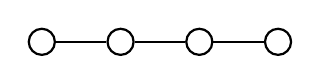
\begin{tikzpicture}[auto,
    specification/.style ={circle, draw, thick}]
   \node[specification] (A) at (0,0)  {};
   \node[specification] (B)  at (1,0)  {};
   \node[specification] (C)  at (2,0)  {};
   \node[specification] (D) at (3,0)  {};
   \draw[thick] (A) to  (B);
   \draw[thick] (B) to  (C);
   \draw[thick] (C) to  (D);
 \end{tikzpicture}
\end{minipage}
\begin{minipage}{0.5\linewidth}
    \centering
    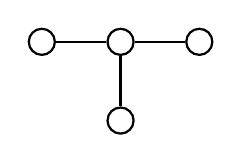
\begin{tikzpicture}[auto,
    specification/.style ={circle, draw, thick}]
   \node[specification] (A) at (0,0)  {};
   \node[specification] (B)  at (1,0)  {};
   \node[specification] (C)  at (2,0)  {};
   \node[specification] (D) at (1,-1)  {};
   \draw[thick] (A) to  (B);
   \draw[thick] (B) to  (C);
   \draw[thick] (B) to  (D);
 \end{tikzpicture}
\end{minipage}

具有$5$个顶点的所有互不同构的树:
  \vspace{0.5cm}

  \begin{minipage}{0.5\linewidth}
    \centering
    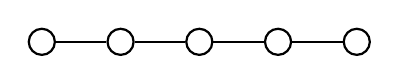
\begin{tikzpicture}[auto,
    specification/.style ={circle, draw, thick}]
   \node[specification] (A) at (0,0)  {};
   \node[specification] (B)  at (1,0)  {};
   \node[specification] (C)  at (2,0)  {};
   \node[specification] (D) at (3,0)  {};
   \node[specification] (E) at (4,0)  {};
   
   \draw[thick] (A) to  (B);
   \draw[thick] (B) to  (C);
   \draw[thick] (C) to  (D);
   \draw[thick] (D) to  (E);
 \end{tikzpicture}
\end{minipage}
  \begin{minipage}{0.5\linewidth}
    \centering
    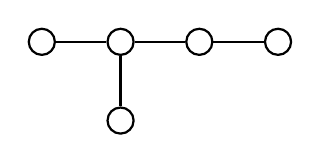
\begin{tikzpicture}[auto,
    specification/.style ={circle, draw, thick}]
   \node[specification] (A) at (0,0)  {};
   \node[specification] (B)  at (1,0)  {};
   \node[specification] (C)  at (2,0)  {};
   \node[specification] (D) at (3,0)  {};
   \node[specification] (E) at (1,-1)  {};
   
   \draw[thick] (A) to  (B);
   \draw[thick] (B) to  (C);
   \draw[thick] (C) to  (D);
   \draw[thick] (B) to (E);
 \end{tikzpicture}
\end{minipage}

  \begin{minipage}{0.5\linewidth}
    \centering
    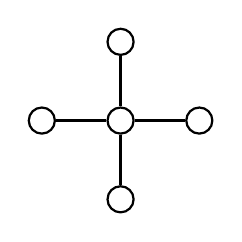
\begin{tikzpicture}[auto,
    specification/.style ={circle, draw, thick}]
   \node[specification] (A) at (0,0)  {};
   \node[specification] (B)  at (1,0)  {};
   \node[specification] (C)  at (2,0)  {};
   \node[specification] (D) at (1,1)  {};
   \node[specification] (E) at (1,-1)  {};
   
   \draw[thick] (A) to  (B);
   \draw[thick] (B) to  (C);
   \draw[thick] (B) to  (D);
   \draw[thick] (B) to (E);
 \end{tikzpicture}
\end{minipage}



具有$6$个顶点的所有互不同构的树:
  \vspace{0.5cm}

  \begin{minipage}{0.5\linewidth}
    \centering
    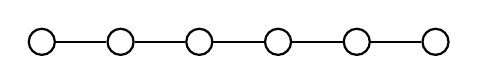
\begin{tikzpicture}[auto,
    specification/.style ={circle, draw, thick}]
   \node[specification] (A) at (0,0)  {};
   \node[specification] (B)  at (1,0)  {};
   \node[specification] (C)  at (2,0)  {};
   \node[specification] (D) at (3,0)  {};
   \node[specification] (E) at (4,0)  {};
   \node[specification] (F) at (5,0)  {};

   \draw[thick] (A) to  (B);
   \draw[thick] (B) to  (C);
   \draw[thick] (C) to  (D);
   \draw[thick] (D) to  (E);
   \draw[thick] (E) to  (F);   
 \end{tikzpicture}
\end{minipage}
  \begin{minipage}{0.5\linewidth}
    \centering
    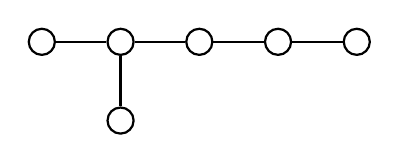
\begin{tikzpicture}[auto,
    specification/.style ={circle, draw, thick}]
   \node[specification] (A) at (0,0)  {};
   \node[specification] (B)  at (1,0)  {};
   \node[specification] (C)  at (2,0)  {};
   \node[specification] (D) at (3,0)  {};
   \node[specification] (E) at (4,0)  {};
   \node[specification] (F) at (1,-1)  {};

   \draw[thick] (A) to  (B);
   \draw[thick] (B) to  (C);
   \draw[thick] (C) to  (D);
   \draw[thick] (D) to  (E);
   \draw[thick] (B) to  (F);   
 \end{tikzpicture}
\end{minipage}

  \begin{minipage}{0.5\linewidth}
    \centering
    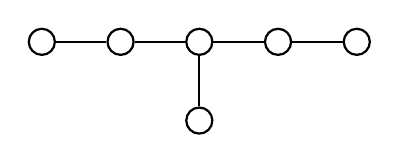
\begin{tikzpicture}[auto,
    specification/.style ={circle, draw, thick}]
   \node[specification] (A) at (0,0)  {};
   \node[specification] (B)  at (1,0)  {};
   \node[specification] (C)  at (2,0)  {};
   \node[specification] (D) at (3,0)  {};
   \node[specification] (E) at (4,0)  {};
   \node[specification] (F) at (2,-1)  {};

   \draw[thick] (A) to  (B);
   \draw[thick] (B) to  (C);
   \draw[thick] (C) to  (D);
   \draw[thick] (D) to  (E);
   \draw[thick] (C) to  (F);   
 \end{tikzpicture}
\end{minipage}
  \begin{minipage}{0.5\linewidth}
    \centering
    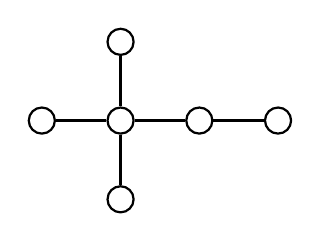
\begin{tikzpicture}[auto,
    specification/.style ={circle, draw, thick}]
   \node[specification] (A) at (0,0)  {};
   \node[specification] (B)  at (1,0)  {};
   \node[specification] (C)  at (2,0)  {};
   \node[specification] (D) at (3,0)  {};
   \node[specification] (E) at (1,1)  {};
   \node[specification] (F) at (1,-1)  {};

   \draw[thick] (A) to  (B);
   \draw[thick] (B) to  (C);
   \draw[thick] (C) to  (D);
   \draw[thick] (B) to  (E);
   \draw[thick] (B) to  (F);   
 \end{tikzpicture}
\end{minipage}

  \begin{minipage}{0.5\linewidth}
    \centering
    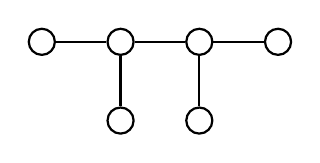
\begin{tikzpicture}[auto,
    specification/.style ={circle, draw, thick}]
   \node[specification] (A) at (0,0)  {};
   \node[specification] (B)  at (1,0)  {};
   \node[specification] (C)  at (2,0)  {};
   \node[specification] (D) at (3,0)  {};
   \node[specification] (E) at (2,-1)  {};
   \node[specification] (F) at (1,-1)  {};

   \draw[thick] (A) to  (B);
   \draw[thick] (B) to  (C);
   \draw[thick] (C) to  (D);
   \draw[thick] (C) to  (E);
   \draw[thick] (B) to  (F);   
 \end{tikzpicture}
\end{minipage}
  \begin{minipage}{0.5\linewidth}
    \centering
    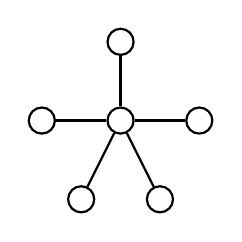
\begin{tikzpicture}[auto,
    specification/.style ={circle, draw, thick}]
   \node[specification] (A) at (0,0)  {};
   \node[specification] (B)  at (1,0)  {};
   \node[specification] (C)  at (2,0)  {};
   \node[specification] (D) at (1,1)  {};
   \node[specification] (E) at (0.5,-1)  {};
   \node[specification] (F) at (1.5,-1)  {};

   \draw[thick] (A) to  (B);
   \draw[thick] (B) to  (C);
   \draw[thick] (B) to  (D);
   \draw[thick] (B) to  (E);
   \draw[thick] (B) to  (F);   
 \end{tikzpicture}
\end{minipage}

  
具有$7$个顶点的所有互不同构的树:
  \vspace{0.5cm}

  \begin{minipage}{0.5\linewidth}
    \centering
    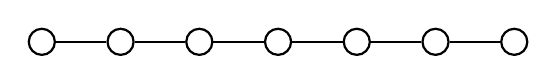
\begin{tikzpicture}[auto,
    specification/.style ={circle, draw, thick}]
   \node[specification] (A) at (0,0)  {};
   \node[specification] (B)  at (1,0)  {};
   \node[specification] (C)  at (2,0)  {};
   \node[specification] (D) at (3,0)  {};
   \node[specification] (E) at (4,0)  {};
   \node[specification] (F) at (5,0)  {};
   \node[specification] (G) at (6,0)  {};

   \draw[thick] (A) to  (B);
   \draw[thick] (B) to  (C);
   \draw[thick] (C) to  (D);
   \draw[thick] (D) to  (E);
   \draw[thick] (E) to  (F);
   \draw[thick] (F) to  (G);   
 \end{tikzpicture}
\end{minipage}
  \begin{minipage}{0.5\linewidth}
    \centering
    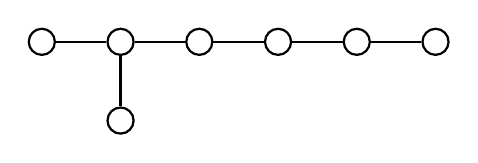
\begin{tikzpicture}[auto,
    specification/.style ={circle, draw, thick}]
   \node[specification] (A) at (0,0)  {};
   \node[specification] (B)  at (1,0)  {};
   \node[specification] (C)  at (2,0)  {};
   \node[specification] (D) at (3,0)  {};
   \node[specification] (E) at (4,0)  {};
   \node[specification] (F) at (5,0)  {};
   \node[specification] (G) at (1,-1)  {};

   \draw[thick] (A) to  (B);
   \draw[thick] (B) to  (C);
   \draw[thick] (C) to  (D);
   \draw[thick] (D) to  (E);
   \draw[thick] (E) to  (F);
   \draw[thick] (B) to  (G);   
 \end{tikzpicture}
\end{minipage}

\vspace{0.5cm}
  \begin{minipage}{0.5\linewidth}
    \centering
    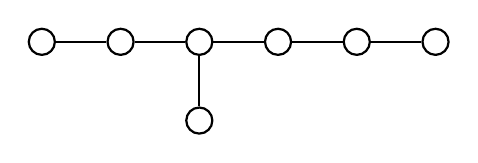
\begin{tikzpicture}[auto,
    specification/.style ={circle, draw, thick}]
   \node[specification] (A) at (0,0)  {};
   \node[specification] (B)  at (1,0)  {};
   \node[specification] (C)  at (2,0)  {};
   \node[specification] (D) at (3,0)  {};
   \node[specification] (E) at (4,0)  {};
   \node[specification] (F) at (5,0)  {};
   \node[specification] (G) at (2,-1)  {};

   \draw[thick] (A) to  (B);
   \draw[thick] (B) to  (C);
   \draw[thick] (C) to  (D);
   \draw[thick] (D) to  (E);
   \draw[thick] (E) to  (F);
   \draw[thick] (C) to  (G);   
 \end{tikzpicture}
\end{minipage}
\begin{minipage}{0.5\linewidth}
    \centering
    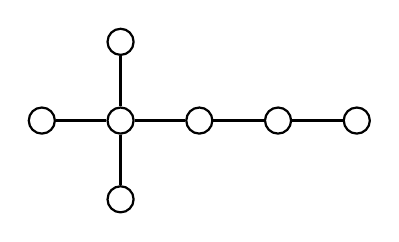
\begin{tikzpicture}[auto,
    specification/.style ={circle, draw, thick}]
   \node[specification] (A) at (0,0)  {};
   \node[specification] (B)  at (1,0)  {};
   \node[specification] (C)  at (2,0)  {};
   \node[specification] (D) at (3,0)  {};
   \node[specification] (E) at (4,0)  {};
   \node[specification] (F) at (1,-1)  {};
   \node[specification] (G) at (1,1)  {};

   \draw[thick] (A) to  (B);
   \draw[thick] (B) to  (C);
   \draw[thick] (C) to  (D);
   \draw[thick] (D) to  (E);
   \draw[thick] (B) to  (F);
   \draw[thick] (B) to  (G);   
 \end{tikzpicture}
\end{minipage}

\vspace{0.5cm}
\begin{minipage}{0.5\linewidth}
    \centering
    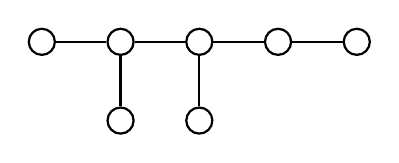
\begin{tikzpicture}[auto,
    specification/.style ={circle, draw, thick}]
   \node[specification] (A) at (0,0)  {};
   \node[specification] (B)  at (1,0)  {};
   \node[specification] (C)  at (2,0)  {};
   \node[specification] (D) at (3,0)  {};
   \node[specification] (E) at (4,0)  {};
   \node[specification] (F) at (1,-1)  {};
   \node[specification] (G) at (2,-1)  {};

   \draw[thick] (A) to  (B);
   \draw[thick] (B) to  (C);
   \draw[thick] (C) to  (D);
   \draw[thick] (D) to  (E);
   \draw[thick] (B) to  (F);
   \draw[thick] (C) to  (G);   
 \end{tikzpicture}
\end{minipage}
\begin{minipage}{0.5\linewidth}
    \centering
    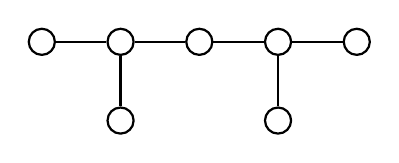
\begin{tikzpicture}[auto,
    specification/.style ={circle, draw, thick}]
   \node[specification] (A) at (0,0)  {};
   \node[specification] (B)  at (1,0)  {};
   \node[specification] (C)  at (2,0)  {};
   \node[specification] (D) at (3,0)  {};
   \node[specification] (E) at (4,0)  {};
   \node[specification] (F) at (1,-1)  {};
   \node[specification] (G) at (3,-1)  {};

   \draw[thick] (A) to  (B);
   \draw[thick] (B) to  (C);
   \draw[thick] (C) to  (D);
   \draw[thick] (D) to  (E);
   \draw[thick] (B) to  (F);
   \draw[thick] (D) to  (G);   
 \end{tikzpicture}
\end{minipage}

\vspace{0.5cm}
\begin{minipage}{0.5\linewidth}
    \centering
    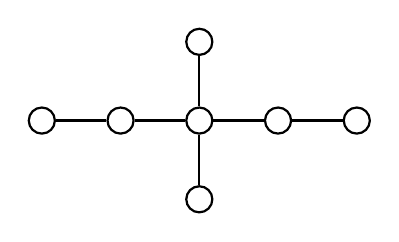
\begin{tikzpicture}[auto,
    specification/.style ={circle, draw, thick}]
   \node[specification] (A) at (0,0)  {};
   \node[specification] (B)  at (1,0)  {};
   \node[specification] (C)  at (2,0)  {};
   \node[specification] (D) at (3,0)  {};
   \node[specification] (E) at (4,0)  {};
   \node[specification] (F) at (2,-1)  {};
   \node[specification] (G) at (2,1)  {};

   \draw[thick] (A) to  (B);
   \draw[thick] (B) to  (C);
   \draw[thick] (C) to  (D);
   \draw[thick] (D) to  (E);
   \draw[thick] (C) to  (F);
   \draw[thick] (C) to  (G);   
 \end{tikzpicture}
\end{minipage}
\begin{minipage}{0.5\linewidth}
    \centering
    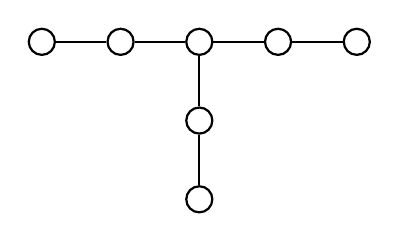
\begin{tikzpicture}[auto,
    specification/.style ={circle, draw, thick}]
   \node[specification] (A) at (0,0)  {};
   \node[specification] (B)  at (1,0)  {};
   \node[specification] (C)  at (2,0)  {};
   \node[specification] (D) at (3,0)  {};
   \node[specification] (E) at (4,0)  {};
   \node[specification] (F) at (2,-1)  {};
   \node[specification] (G) at (2,-2)  {};

   \draw[thick] (A) to  (B);
   \draw[thick] (B) to  (C);
   \draw[thick] (C) to  (D);
   \draw[thick] (D) to  (E);
   \draw[thick] (C) to  (F);
   \draw[thick] (F) to  (G);   
 \end{tikzpicture}
\end{minipage}

\vspace{0.5cm}
  \begin{minipage}{0.5\linewidth}
    \centering
    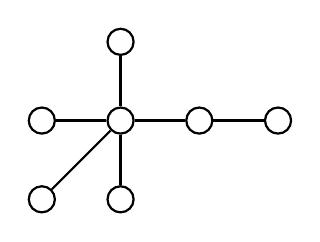
\begin{tikzpicture}[auto,
    specification/.style ={circle, draw, thick}]
   \node[specification] (A) at (0,0)  {};
   \node[specification] (B)  at (1,0)  {};
   \node[specification] (C)  at (2,0)  {};
   \node[specification] (D) at (3,0)  {};
   \node[specification] (E) at (1,1)  {};
   \node[specification] (F) at (0,-1)  {};
   \node[specification] (G) at (1,-1)  {};

   \draw[thick] (A) to  (B);
   \draw[thick] (B) to  (C);
   \draw[thick] (C) to  (D);
   \draw[thick] (B) to  (E);
   \draw[thick] (B) to  (F);
   \draw[thick] (B) to  (G);   
 \end{tikzpicture}
\end{minipage}
  \begin{minipage}{0.5\linewidth}
    \centering
    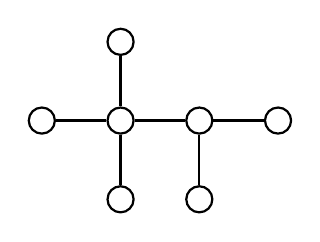
\begin{tikzpicture}[auto,
    specification/.style ={circle, draw, thick}]
   \node[specification] (A) at (0,0)  {};
   \node[specification] (B)  at (1,0)  {};
   \node[specification] (C)  at (2,0)  {};
   \node[specification] (D) at (3,0)  {};
   \node[specification] (E) at (1,1)  {};
   \node[specification] (F) at (2,-1)  {};
   \node[specification] (G) at (1,-1)  {};

   \draw[thick] (A) to  (B);
   \draw[thick] (B) to  (C);
   \draw[thick] (C) to  (D);
   \draw[thick] (B) to  (E);
   \draw[thick] (C) to  (F);
   \draw[thick] (B) to  (G);   
 \end{tikzpicture}
\end{minipage}

\vspace{0.5cm}
  \begin{minipage}{0.5\linewidth}
    \centering
    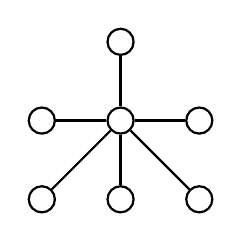
\begin{tikzpicture}[auto,
    specification/.style ={circle, draw, thick}]
   \node[specification] (A) at (0,0)  {};
   \node[specification] (B)  at (1,0)  {};
   \node[specification] (C)  at (2,0)  {};
   \node[specification] (D) at (1,1)  {};
   \node[specification] (E) at (0,-1)  {};
   \node[specification] (F) at (1,-1)  {};
   \node[specification] (G) at (2,-1)  {};

   \draw[thick] (A) to  (B);
   \draw[thick] (B) to  (C);
   \draw[thick] (B) to  (D);
   \draw[thick] (B) to  (E);
   \draw[thick] (B) to  (F);
   \draw[thick] (B) to  (G);   
 \end{tikzpicture}
\end{minipage}

  
\end{proof}
